\section{Results}

The purpose of this thesis work was to design and implement an interactive and semi automated web based tool for discovering association rules from the Carat data that indicate what system settings and usage patterns of a mobile application lead to increased battery consumption. In practise, this has proven to be quite challenging for a number of reasons:

\begin{itemize}
  \item Automatically deciding a sufficient threshold for support and confidence for generating rules is difficult 
  \item Number of generated rules increases rapidly as support and confidence thresholds are lowered
  \item Identifying interesting or relevant rules in presence of hundreds or thousands of rules is cumbersome
  \item Deciding how to discretize ordinal and continuous variables is non-trivial          
\end{itemize}

We will now look at the results of this work in two parts. In the first part we will be looking at the performance of the application and how it affects its usability. In the second part we will take a look at some example use cases of the system.  

\subsection{Performance Evaluation}

\begin{figure}[htp]

\subfloat[Number of rules with fitted plane]{
  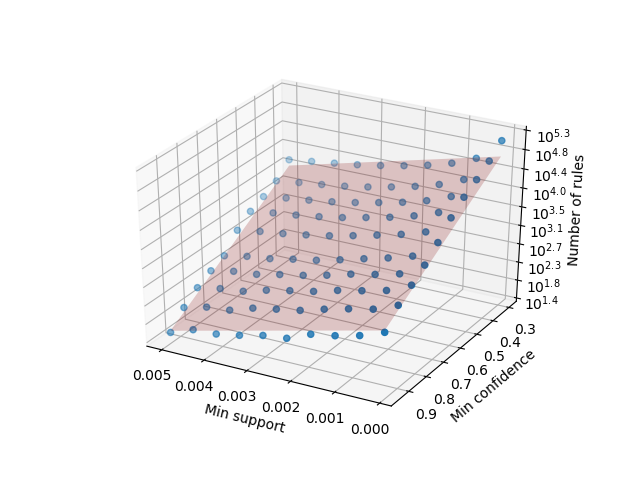
\includegraphics[width=\textwidth]{images/results/facebook_num_rules.png}%
}

\subfloat[Number of rules with error bars]{%
  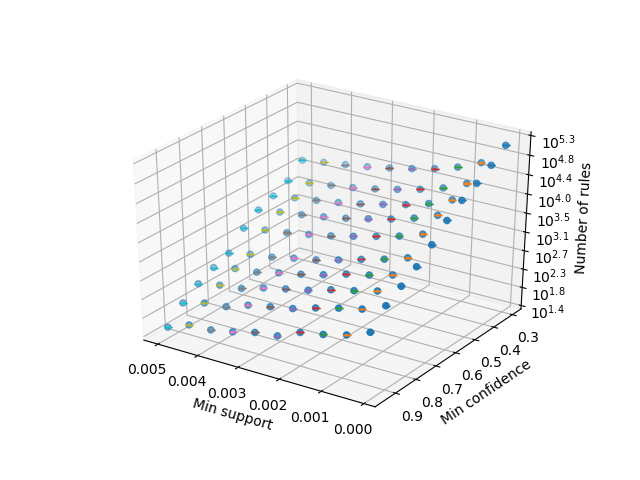
\includegraphics[width=\textwidth]{images/results/facebook_num_rules_with_error_bars.png}%
}

\caption{Number of generated rules for Facebook measurements as a function of minimum support threshold and minimum confidence threshold}
\label{figure:number-of-rules-facebook}
\end{figure}

In order to understand the relationship between the number of generated rules and minimum support and confidence thresholds, a series of measurements were conducted on the Carat API prototype server. Figure~\ref{figure:number-of-rules-facebook} shows these  measurements for Facebook application and Figure~\ref{figure:number-of-rules-spotify} shows the measurements for Spotify application. The figures show the relationship of generated rules as a function of minimum support threshold and confidence threshold as a three dimensional plot. A series of five measurements were conducted for each application. In each of series, a minimum confidence threshold range of 0.3 to 0.9 and a minimum support threshold range of 0.0001 to 0.005 were both divided evenly by 10 points creating a grid of 100 points where the measurements were taken. The blue dots represent average of the five measurement at each point of the support-confidence-grid. In sub figure A, a plane was fitted to the measurements points using least squares method. This was done to better illustrate the spatial configuration of the measurements as well as to showcase how well the measured points are aligned on the plane. In sub figure B, error bars were plotted to the measurements using one standard deviation of the five measurements as the size of the error. 

%Figure~\ref{figure:number-of-ruless} shows the relationship of these variables on two selected applications, namely Spotify and Facebook mobile applications. The blue dots represent individual measurements. A minimum confidence threshold range of 0.3 to 0.9 and a minimum support threshold range of 0.0001 to 0.005 were both divided evenly by 10 points creating a grid of 100 points where the measurements were taken. The number of rules -axis is in $log_{10}$ scale to better illustrate the varying magnitudes of the number of generated rules. The transparent red plane was fitted to the measured points using the least squares method.

The number generated rules seems to grow exponentially on both axes when approaching zero, as can be seen by how well the measurements align with the least squares plane. This explosion in the number of generated rules makes it difficult for the user to extract useful rules from the system when small values for the thresholds are used. To mitigate this problem, the system provides two features:

\begin{itemize}
	\item The generated rules are sorted in the ascending order of their confidence, giving the more reliable rules a greater priority.    
         
	\item Attributes can be excluded from the analysis - potentially greatly reducing the number of generated rules. 
\end{itemize}        

Even though there is a stochastic component in the rule generation, which arises from the sampling of data in the variable discretization stage of the analysis, the number of generated rules does not seem to vary much, as can be seen from the error bars, which are barely visible.  


\begin{figure}[htp]
\subfloat[Number of rules with fitted plane]{
  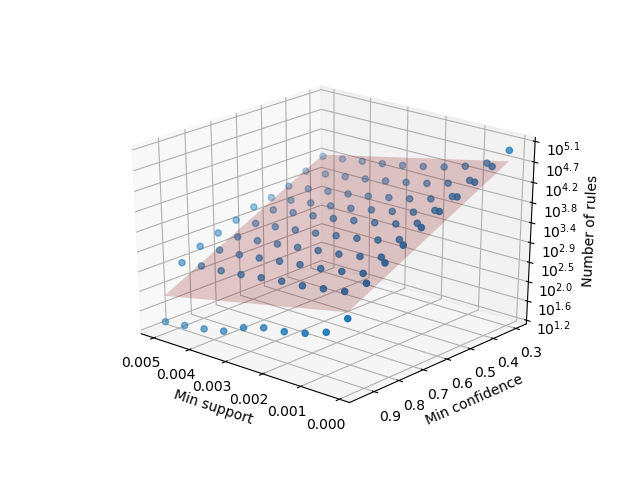
\includegraphics[width=\textwidth]{images/results/spotify_num_rules.png}%
}

\subfloat[Number of rules with error bars]{%
  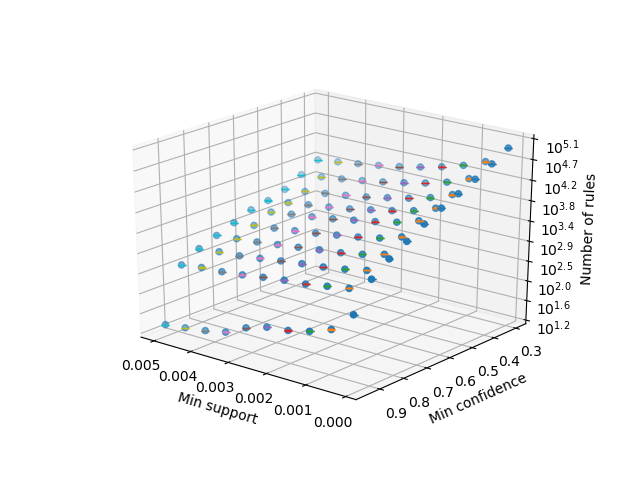
\includegraphics[width=\textwidth]{images/results/spotify_num_rules_with_error_bars.png}%
}

\caption{Number of generated rules for Spotify measurements as a function of minimum support threshold and minimum confidence threshold}
\label{figure:number-of-rules-spotify}
\end{figure}


%\begin{figure}[htp]
%\subfloat[Facebook mobile application]{%
%  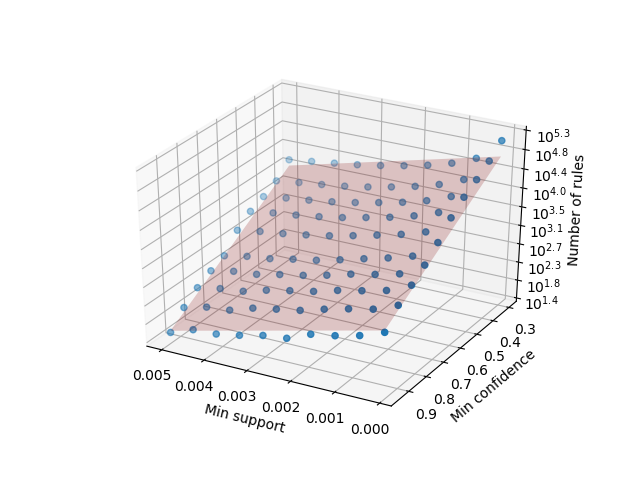
\includegraphics[width=\textwidth]{images/results/facebook_num_rules.png}%
%}
%\subfloat[Spotify mobile application]{%
%  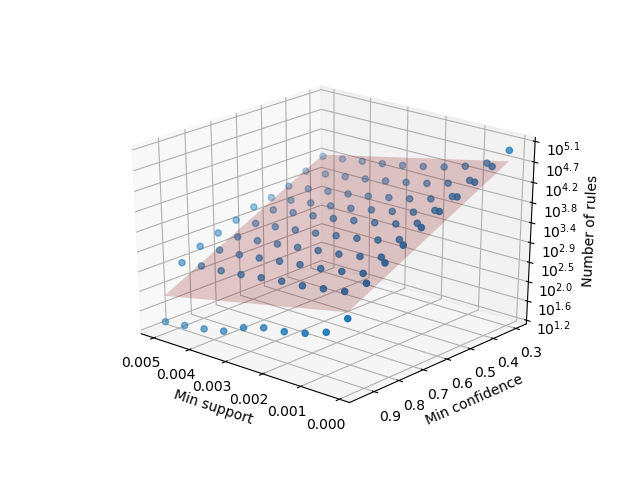
\includegraphics[width=\textwidth]{images/results/spotify_num_rules.png}%
%}
%\caption{Number of generated rules plotted as a function of minimum support threshold and minimum confidence threshold}
%\label{figure:number-of-ruless}
%\end{figure}

\begin{figure}[htp]

\subfloat[Rule generation time with best fitting plane]{
  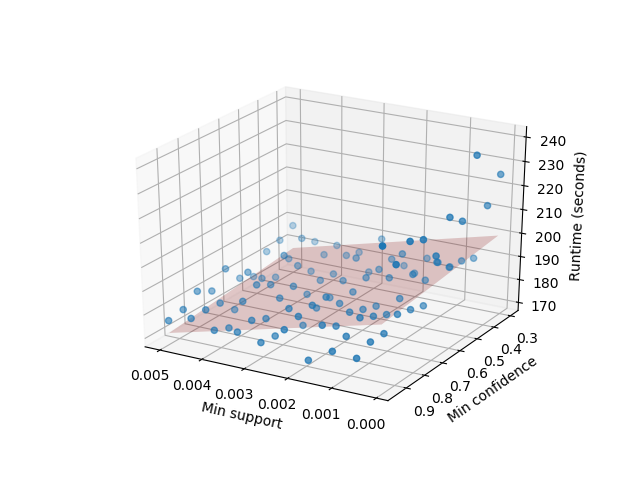
\includegraphics[width=\textwidth]{images/results/facebook_runtimes.png}%
}

\subfloat[Rule generation time with error bars]{%
  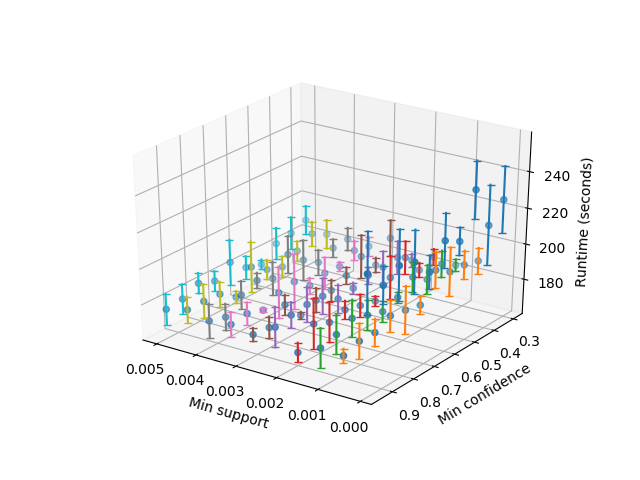
\includegraphics[width=\textwidth]{images/results/facebook_runtimes_with_error_bars.png}%
}

\caption{Rule generation time for Facebook measurements as a function of minimum support threshold and minimum confidence threshold}
\label{figure:runtimes-facebook}
\end{figure}

In addition to the number of generated rules, another metric that is a good indicator for usability of the system, is the time taken to generate the association rules. To measure the time of the rule generation as a function of minimum support threshold and minimum confidence threshold, a similar set up as with the number of generated rules was used. Figure~\ref{figure:runtimes-facebook} shows these measurements for the Facebook application and Figure~\ref{figure:runtimes-spotify} shows the measurements for the Spotify application. Like before, the blue dots represent the average value in five measurements series of 100 measurement points. The red plane represents a plane that was fitted to the points using the least squares method. The size of the error in the error bars is again the standard deviation of the measurement at each measurement point.

The rule generation time increases as either axis approaches zero. The deviance is not huge however, as all the measured run times fall between 160 and 260 seconds. While this is a notable difference from the users perspective, the system remains usable even when the number of generated rules is in the order of $10^5$.   

\begin{figure}[htp]

\subfloat[Rule generation time with best fitting plane]{
  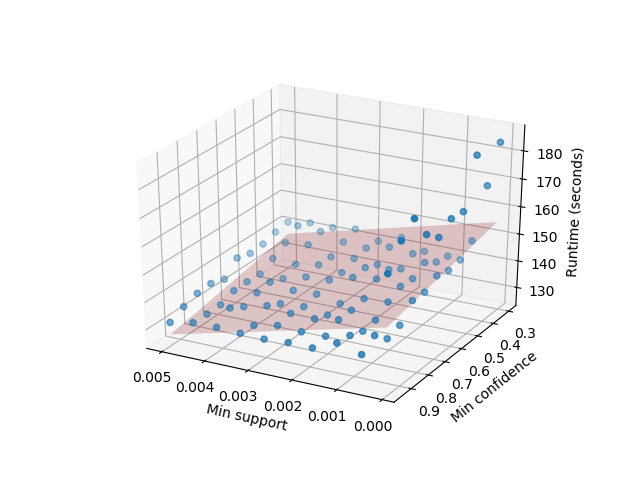
\includegraphics[width=\textwidth]{images/results/spotify_runtimes.png}%
}

\subfloat[Rule generation time with error bars]{%
  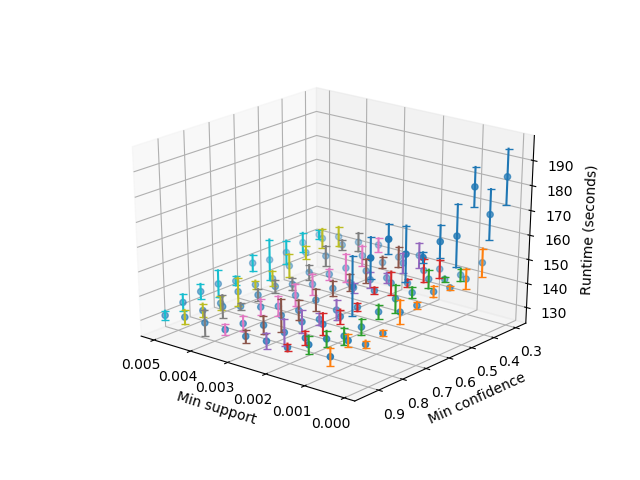
\includegraphics[width=\textwidth]{images/results/spotify_runtimes_with_error_bars.png}%
}

\caption{Rule generation time for Spotify measurements as a function of minimum support threshold and minimum confidence threshold}
\label{figure:runtimes-spotify}
\end{figure}

All the experiments were conducted on a Spark cluster which had a single computing server. For each run, 45 CPU cores and 1500 gigabytes of memory were reserved. To mitigate the effect effect of any potential file server load, the dataset was stored in memory using Linux shared memory file system (/dev/shm). The dataset consisted of Carat samples from 22.6.2016 to 22.8.2016, the size of which was a little over 16 gigabytes.


%\begin{figure}[htp]
%\subfloat[Facebook mobile application]{%
%  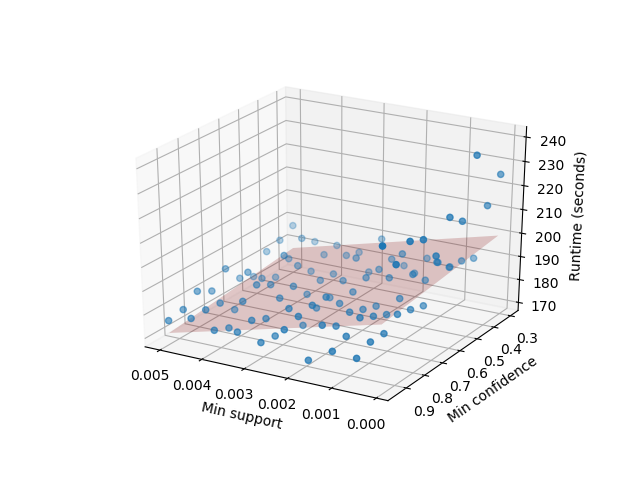
\includegraphics[width=\textwidth]{images/results/facebook_runtimes.png}%
%}
%\subfloat[Spotify mobile application]{%
%  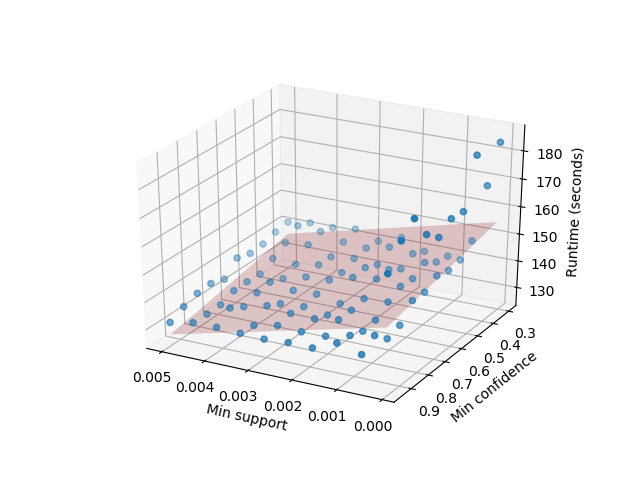
\includegraphics[width=\textwidth]{images/results/spotify_runtimes.png}%
%}
%\caption{Association rule generation time as a function of minimum support threshold and minimum confidence threshold}
%\label{figure:analysis-runtime}
%\end{figure}  

\subsection{Overview on Generated Rules}